\chapter{群速度、費米子排斥與狄拉克海}

\section{相速度與群速度}

\begin{classroomqa}
\lecturetimestamp{00:00:07}
\audiencequestion{什麼是群速度和相速度？}
\lecturerresponse{相速度描述平面波中相位固定點的移動，通常並不代表可測量物體的運動。群速度描述波包包絡的移動，是與粒子、訊號及機率流相關的速度。}
\end{classroomqa}

先從平面波開始，
\begin{equation}
\psi(x,t)=e^{i(kx-\omega t)},
\end{equation}
或從它的實數形式開始，
\begin{equation}
\psi(x,t)=\sin(kx-\omega t).
\end{equation}
波峰、波谷或任何其他相位固定點的移動滿足
\begin{equation}
kx-\omega t=\text{constant}.
\end{equation}
為了方便，令這個常數為零，得到
\begin{equation}
x=\frac{\omega}{k}t,
\qquad
v_{\mathrm{phase}}=\frac{\omega}{k}.
\end{equation}
由於 \(\omega=2\pi/T\) 且 \(k=2\pi/\lambda\)，
\begin{equation}
v_{\mathrm{phase}}=\frac{\omega}{k}=\frac{\lambda}{T}.
\end{equation}
這正是一個固定相位在一個週期內前進的距離。

對於非相對論性的 Schr\"odinger 波，取 \(\hbar=1\)，能量與動量分別為 \(\omega\) 和 \(k\)，因此
\begin{equation}
\omega(k)=\frac{k^2}{2m}.
\end{equation}
其相速度為
\begin{equation}
v_{\mathrm{phase}}=\frac{k}{2m}.
\end{equation}
然而，動量為 \(k\) 的粒子，其一般速度為 \(k/m\)。這個相差二倍的結果，首先提醒我們：平面波相位的移動並不等於粒子的移動。

還有一個更明確的警訊。對每個頻率都加上同一個常數 \(C\)：
\begin{equation}
\omega(k)\longrightarrow \omega(k)+C.
\end{equation}
例如，這個常數可以代表共同的靜止能量貢獻，如 \(mc_{\mathrm{light}}^2\)；但它具體代表什麼並不重要。此處的 \(C\) 是能量偏移量，不是光速。相速度會變成
\begin{equation}
v_{\mathrm{phase}}\longrightarrow
\frac{\omega(k)+C}{k}
=v_{\mathrm{phase}}+\frac{C}{k}.
\end{equation}
然而，對每個能量都加上同一個常數，不會改變任何能量差，因此也不會改變非相對論物理。

從波函數可以直接看出這一點。將一般的 Schr\"odinger 場寫成各模式的總和或積分，
\begin{equation}
\psi(x,t)=\sum_k a_k e^{ikx}e^{-i\omega(k)t},
\end{equation}
其中省略了正規化因子。平移之後，
\begin{align}
\psi(x,t)
&\longrightarrow
\sum_k a_k e^{ikx}e^{-i[\omega(k)+C]t}
\\
&=e^{-iCt}\psi(x,t).
\end{align}
每個模式都獲得相同的時間相依相位。共軛場則獲得相反的相位，因此
\begin{equation}
\begin{aligned}
\psi^*(x,t)\psi(x,t)
&\longrightarrow
e^{iCt}e^{-iCt}\psi^*(x,t)\psi(x,t)
\\
&=\psi^*(x,t)\psi(x,t).
\end{aligned}
\end{equation}
期望值中也會發生同樣的抵消。若某個量會因能量零點平移而改變，它就不可能是 Schr\"odinger 粒子的物理傳播速度。因此，相速度有一部分取決於約定。

局域化粒子不是以單一無限延伸的平面波表示，而是以波包表示。各分量波在波包所在區域相長干涉，在區域之外相消干涉。僅考察兩個相近的波，就能求出這個干涉圖樣的移動：
\begin{equation}
\psi(x,t)=
\sin(kx-\omega t)+
\sin(k'x-\omega't),
\end{equation}
其中 \(k'\) 接近 \(k\)，且 \(\omega'=\omega(k')\)。相位相同之處會形成相長干涉的軌跡，
\begin{equation}
kx-\omega t=k'x-\omega't.
\end{equation}
因此
\begin{equation}
(k-k')x=(\omega-\omega')t,
\end{equation}
增強的干涉圖樣便依照下式移動：
\begin{equation}
x=\frac{\omega-\omega'}{k-k'}t.
\end{equation}
令兩個波彼此無限接近，得到
\begin{equation}
x=\frac{d\omega}{dk}t,
\qquad
v_{\mathrm{group}}=\frac{d\omega}{dk}.
\end{equation}
這就是包絡的速度---也就是分量波干涉所形成之局域波包的速度。

對於含有任意偏移量的非相對論色散關係，
\begin{equation}
\omega(k)=\frac{k^2}{2m}+C,
\end{equation}
群速度為
\begin{equation}
v_{\mathrm{group}}
=\frac{d}{dk}\left(\frac{k^2}{2m}+C\right)
=\frac{2k}{2m}
=\frac{k}{m}.
\end{equation}
加法常數消失了，結果恰好就是經典粒子的速度。

\begin{classroomqa}
\lecturetimestamp{00:16:35}
\audiencequestion{群速度中的二倍因子會消失嗎？}
\lecturerresponse{會。對 \(k^2\) 微分會得到 \(2k\)，恰好抵消 \(2m\) 中的二，因此結果是 \(k/m\)。}
\end{classroomqa}

因此，群速度是最接近經典粒子運動的速度，也是描述波包傳播的相關速度；在此處考慮的一般情形下，它也與訊號傳播有關。相速度則不一定具有上述任一含義。

\subsection{無質量與有質量的相對論性波}

\begin{classroomqa}
\lecturetimestamp{00:17:47}
\audiencequestion{這和「光能比光傳得更快」的說法有關嗎？}
\lecturerresponse{沒有。那些說法涉及另一個問題。相關計算確實顯示，相位可以比光速移動得更快，而物理上的群速度仍低於光速；但這不代表訊號超越光速。}
\end{classroomqa}

\begin{classroomqa}
\lecturetimestamp{00:18:05}
\audiencequestion{相關例子是不是大家熟悉的那種：相速度超過光速，而群速度仍低於光速？}
\lecturerresponse{是的。具有非零質量的相對論性波也呈現同樣的情形，這可直接由相對論性能量--動量關係推出。}
\end{classroomqa}

令 \(\hbar=c_{\mathrm{light}}=1\)。相對論關係為
\begin{equation}
E=\sqrt{p^2+m^2},
\qquad
\omega(k)=\sqrt{k^2+m^2}.
\end{equation}
先考察無質量的情形會很有幫助。當 \(m=0\) 時，
\begin{equation}
\omega=|k|.
\end{equation}
在向右傳播的分支 \(k>0\) 上，\(\omega=k\)，因此
\begin{equation}
v_{\mathrm{phase}}=\frac{\omega}{k}=1,
\qquad
v_{\mathrm{group}}=\frac{d\omega}{dk}=1.
\end{equation}
在向左傳播的分支上，兩種速度則都帶有相應的負號。無論哪一種情形，速度大小都是光速。由於色散關係在各分支上都是線性的，同一分支上的所有傅立葉分量都以相同速度傳播。

對於 \(k>0\) 的有質量粒子，
\begin{equation}
v_{\mathrm{phase}}
=\frac{\omega}{k}
=\sqrt{\frac{k^2+m^2}{k^2}}>1,
\end{equation}
而
\begin{equation}
v_{\mathrm{group}}
=\frac{d\omega}{dk}
=\frac{k}{\sqrt{k^2+m^2}}<1.
\end{equation}
當 \(k<0\) 時，兩種速度都反號，但其大小仍滿足相同的不等式。因此，相位可以比光速移動得更快，而波包、粒子、能量與訊號則以低於光速的速度移動。對於這個特定的色散關係，在 \(k\neq0\) 時，
\begin{equation}
v_{\mathrm{phase}}v_{\mathrm{group}}=1.
\end{equation}
這種互為倒數的關係是平方根色散關係的特例，並非波的一般性質。

\begin{figure}
\centering
\includegraphics[width=0.72\textwidth]{lecture_05_figure_03.png}
\caption{非相對論性與相對論性色散關係；相速度為 \(\omega/k\)，群速度為 \(d\omega/dk\)。}
\lectureframe{00:35:52}
\end{figure}

\begin{classroomqa}
\lecturetimestamp{00:23:41}
\audiencequestion{色散是否表示波速會隨頻率改變？}
\lecturerresponse{是的。當 \(\omega(k)\) 是線性的，每個傅立葉分量的群速度都相同，波包便能保持形狀。當 \(\omega(k)\) 是非線性的，不同分量會以不同速度傳播，因此波包會色散並改變形狀。若低頻聲波的頻率近似正比於波數，它便近似不具色散。}
\end{classroomqa}

一般而言，相速度既不傳遞訊號，也不傳遞能量或機率流。只要平移能量零點，它的數值甚至就會改變。對於足夠窄的波包，群速度才是具有物理意義的傳播速度。

\begin{classroomqa}
\lecturetimestamp{00:25:14}
\audiencequestion{光子的相速度可以測量嗎？}
\lecturerresponse{在真空中，光子的色散關係是線性的，因此相速度和群速度相同，兩者都等於光速。在物質介質中，色散關係會改變，相速度和群速度便不一定相同。}
\end{classroomqa}

\begin{classroomqa}
\lecturetimestamp{00:25:50}
\audiencequestion{這裡的討論是否只適用於不隨時間展寬的波包？}
\lecturerresponse{只有在波包的所有傅立葉分量都具有相同速度時，波包才不會展寬；這對應於相關範圍內的線性色散關係。若色散關係是非線性的，各分量便會逐漸分離，波包也會展寬。}
\end{classroomqa}

光錐與相對論因果結構的問題，光靠區分相速度與群速度並不足以處理，因此不在這項計算中討論。

\section{平移對稱性與守恆定律}

同樣的平面波相位可以簡潔地說明守恆定律。先從能量守恆談起。湮滅場作用於能量為 \(\omega_j\) 的入射粒子時，會帶來時間因子
\begin{equation}
e^{-i\omega_j t},
\end{equation}
而產生能量為 \(\omega'_r\) 的出射粒子時，產生場會帶來
\begin{equation}
e^{+i\omega'_r t}.
\end{equation}
若有多個入射粒子與出射粒子，這些因子的乘積為
\begin{equation}
\exp\!\left[
i\left(\sum_r\omega'_r-\sum_j\omega_j\right)t
\right].
\end{equation}
若相互作用在任何時刻發生的振幅都相同，振幅中便會包含對相互作用時間的積分：
\begin{equation}
\begin{aligned}
&\int_{-\infty}^{\infty}dt\,
\exp\!\left[
i\left(\sum_r\omega'_r-\sum_j\omega_j\right)t
\right]
\\
&\quad =2\pi\,
\delta\!\left(\sum_r\omega'_r-\sum_j\omega_j\right).
\end{aligned}
\end{equation}
{\proseunicodefont δ} 函數要求出射粒子的總能量等於入射粒子的總能量。任一可能相互作用時刻的振幅皆相同，這就是時間平移不變性，而它導出能量守恆。

空間平移也以相同機制導出動量守恆。考慮一個物理的一變二衰變：動量為 \(k\) 的入射粒子消失，並出現兩個動量分別為 \(k'_1\) 和 \(k'_2\) 的粒子。位於 \(x\) 的局域相互作用包含一個湮滅場和兩個產生場，
\begin{equation}
\mathcal{O}(x)=\psi^\dagger(x)\psi^\dagger(x)\psi(x).
\end{equation}
略去時間相依性與正規化因子後，相關的模式因子為
\begin{align}
\psi(x)&\supset a_k e^{ikx},
\\
\psi^\dagger(x)&\supset a_{k'_1}^\dagger e^{-ik'_1x},
\qquad
\psi^\dagger(x)\supset a_{k'_2}^\dagger e^{-ik'_2x}.
\end{align}
在矩陣元素
\begin{equation}
\langle k'_1,k'_2|\mathcal{O}(x)|k\rangle,
\end{equation}
中，湮滅算符移除入射粒子，兩個產生算符則產生出射粒子。這些算符作用完成後，留下的位置相依因子為
\begin{equation}
e^{-ik'_1x}e^{-ik'_2x}e^{ikx}
=e^{i(k-k'_1-k'_2)x}.
\end{equation}
由於沒有任何位置具有特殊地位，必須對所有可能的衰變位置積分：
\begin{equation}
\int_{-\infty}^{\infty}dx\,
e^{i(k-k'_1-k'_2)x}
=2\pi\delta(k-k'_1-k'_2).
\end{equation}
因此，非零振幅必須滿足
\begin{equation}
k=k'_1+k'_2.
\end{equation}
在三維空間中，同樣的計算會使用 \(d^3x\)、粗體表示的動量向量，以及三維 {\proseunicodefont δ} 函數。這個論證並不依賴只有一個入射粒子或兩個出射粒子。對任意數目的粒子，對共同的相互作用位置積分便會得到
\begin{equation}
\delta^{(3)}\!\left(
\sum_j\mathbf{k}_j-\sum_r\mathbf{k}'_r
\right).
\end{equation}
每個位置的振幅都相同，就是空間平移不變性；它導出動量守恆，正如每個時刻的振幅都相同會導出能量守恆。

第三個例子是整體相位旋轉，
\begin{equation}
\psi\longrightarrow e^{i\lambda}\psi,
\qquad
\psi^\dagger\longrightarrow e^{-i\lambda}\psi^\dagger.
\end{equation}
若相互作用振幅中湮滅場與產生場所帶來的相位彼此抵消，振幅便保持不變。對於帶電場，這表示初態中移除的電荷等於末態中補回的電荷，也就是電荷守恆。因此，時間平移、空間平移與整體相位旋轉說明了場如何透過產生和湮滅粒子，表現能量、動量與電荷守恆。

\begin{classroomqa}
\lecturetimestamp{00:37:52}
\audiencequestion{對空間積分，是指對全部三個空間維度積分嗎？}
\lecturerresponse{是的。三個積分會產生一個涵蓋三個動量分量的 {\proseunicodefont δ} 函數，因此總動量的三個分量都守恆。}
\end{classroomqa}

\begin{classroomqa}
\lecturetimestamp{00:38:03}
\audiencequestion{這個模型能決定守恆動量以不同方式分配時，各種情形的相對機率嗎？}
\lecturerresponse{不能。這個簡單的表示式只要求出射動量的總和符合條件，並不偏向任何特定的分配方式。要決定相對機率，還需要額外的動力學資訊。}
\end{classroomqa}

\begin{classroomqa}
\lecturetimestamp{00:39:04}
\audiencequestion{為什麼湮滅算符的總和會只留下與佔據動量相符的那一項？}
\lecturerresponse{湮滅算符作用在空模式上會得到零向量。若態中只有一個粒子，而且它只佔據模式 \(k_0\)，除了 \(k=k_0\) 的那一項之外，其餘各項都會消失。}
\end{classroomqa}

例如，
\begin{equation}
\sum_k a_k e^{ikx}|1_{k_0}\rangle
=e^{ik_0x}|0\rangle,
\end{equation}
略去正規化因子後即為此式：所有對應空模式的湮滅算符作用後，都會得到零向量。

\section{玻色子增強與費米子排斥}

玻色子在單粒子態中的佔據數可以是任意非負整數，而且玻色子的產生算符代數確實會增強已被佔據的態。對單一玻色模式，標準的正規化數態記號將佔據增強寫成\footnote{講義說明了佔據數平方根形式的增強；此處編號的方程式則是標準的數態寫法。}
\begin{equation}
a^\dagger|n\rangle=\sqrt{n+1}\,|n+1\rangle.
\end{equation}
假設一個處於激發態的原子可以向許多可能模式之一發射光子。若沒有其他光子，各個方向與動量的出現機率就遵循通常的分布。若某一模式中已經有許多光子---而且它們的動量、能量與頻率都相同---，向該模式發射光子的機率便會因相應的佔據數平方根因子而增強。原子會傾向將光子加入已經有光子的態中。這就是受激發射，也是玻色子聚集的具體表現。

費米子的行為正好相反。兩個全同費米子不能佔據同一個量子態。泡利不相容原理最初是在原子物理中提出的：原子中的兩個電子不能具有完全相同的量子數。但這項原理不限於原子；在任何地方，全同費米子都不能共享同一個完整的單粒子態。

場的展開一開始看起來和玻色子的展開完全一樣。在有限大小的盒子中，可以寫成
\begin{equation}
\psi(x)=\sum_k A_k e^{ikx},
\qquad
\psi^\dagger(x)=\sum_k A_k^\dagger e^{-ikx}.
\end{equation}
對連續動量而言，總和則改為積分。共軛場展開中的空間相位帶有相反符號，這是厄米共軛的結果。這部分的建構屬於非相對論情形；相對論性費米子要到最後才會登場。

場的狀態仍以每個模式的佔據數記錄，但現在每個佔據數只能是零或一：
\begin{equation}
|n_{k_1},n_{k_2},\ldots\rangle,
\qquad n_k\in\{0,1\}.
\end{equation}
不存在其他相對論性粒子類型，例如每個態至多能有三個粒子，或至少要有七個粒子。要證明玻色統計與費米統計是僅有的可能性，還需要結合量子力學與狹義相對論，這超出本次討論的範圍。此處要做的是描述費米子的可能性及其後果。

\subsection{單一費米子態}

聚焦於單一粒子的狀態。它不是空態 \(|0\rangle\)，就是佔據態 \(|1\rangle\)。產生與湮滅算符的作用如下：
\begin{align}
A^\dagger|0\rangle&=|1\rangle,
&
A^\dagger|1\rangle&=0,
\\
A|0\rangle&=0,
&
A|1\rangle&=|0\rangle.
\end{align}
右側未加修飾的零表示零向量，不是空態 \(|0\rangle\)。試圖再加入一個費米子，並不會得到真空態；結果是根本沒有任何物理態。

\begin{classroomqa}
\lecturetimestamp{00:46:25}
\audiencequestion{費米子的產生與湮滅算符仍然是線性算符嗎？}
\lecturerresponse{是的。量子力學中的算符都是線性算符，費米子的產生與湮滅算符也不例外。}
\end{classroomqa}

\begin{classroomqa}
\lecturetimestamp{00:47:34}
\audiencequestion{零是指空態，還是指這項操作無法產生任何態？}
\lecturerresponse{它表示零向量，不是空態。真正的真空態或基態具有非零波函數；恆等於零的函數範數為零，因此不是物理態。}
\end{classroomqa}

諧振子讓這項區分變得具體。它的基態，也就是沒有振子激發的狀態，具有如下形式的高斯波函數：
\begin{equation}
\phi_0(q)\propto e^{-\alpha q^2},
\qquad \alpha>0.
\end{equation}
這是完全合理且可正規化的量子態。相較之下，
\begin{equation}
\phi(q)\equiv0
\end{equation}
是零向量：它在任何位置都沒有機率振幅，因此不是量子態。所以 \(A^\dagger|1\rangle=0\) 表示試圖進行第二次產生時，結果是零向量。

\begin{classroomqa}
\lecturetimestamp{00:48:42}
\audiencequestion{費米子算符是否應該使用不同於玻色子算符的記號？}
\lecturerresponse{是的。將 \(a\) 和 \(a^\dagger\) 保留給玻色模式，並用 \(c\) 和 \(c^\dagger\) 表示費米模式，會更清楚。文獻中兩種記號都有人使用，但採用不同字母可清楚區分兩種代數。}
\end{classroomqa}

採用這套記號後，單一模式的規則為
\begin{align}
c^\dagger|0\rangle&=|1\rangle,
&c^\dagger|1\rangle&=0,
\\
c|0\rangle&=0,
&c|1\rangle&=|0\rangle.
\end{align}
接著在兩個基底態上分別計算兩種可能的乘積。在空態上，
\begin{align}
c^\dagger c|0\rangle&=0,
&
cc^\dagger|0\rangle&=|0\rangle.
\end{align}
在佔據態上，
\begin{align}
c^\dagger c|1\rangle&=|1\rangle,
&
cc^\dagger|1\rangle&=0.
\end{align}
兩者相加後，會得到它們作用的那個態：
\begin{align}
(c^\dagger c+cc^\dagger)|0\rangle&=|0\rangle,
\\
(c^\dagger c+cc^\dagger)|1\rangle&=|1\rangle.
\end{align}
由於 \(|0\rangle\) 和 \(|1\rangle\) 張成單一模式的態空間，
\begin{equation}
c^\dagger c+cc^\dagger=1.
\end{equation}
帶正號的組合稱為反對易子，
\begin{equation}
\{A,B\}=AB+BA,
\end{equation}
所以費米子的關係式為
\begin{equation}
\{c,c^\dagger\}=1.
\end{equation}
這是玻色子對易子
\begin{equation}
[a,a^\dagger]=aa^\dagger-a^\dagger a=1.
\end{equation}
的費米子類比。

對同一費米子態進行兩次產生，結果必為零。若該態原本是空的，第一次產生會將它填滿，第二次便無法再產生；若它原本已被佔據，第一次產生就已經無法進行。兩次湮滅也必為零。因此
\begin{equation}
\{c^\dagger,c^\dagger\}=2(c^\dagger)^2=0,
\qquad
\{c,c\}=2c^2=0.
\end{equation}

\begin{classroomqa}
\lecturetimestamp{00:56:45}
\audiencequestion{湮滅算符平方關係式中的零，是指零向量嗎？}
\lecturerresponse{這個方程式表示 \(c^2\) 是零算符，也就是會將每個態向量都映射為零向量的算符。零算符與零向量是不同的數學物件，雖然前者作用後總會得到後者。}
\end{classroomqa}

對於許多離散動量模式，完整的代數關係為
\begin{align}
\{c_k,c_{k'}^\dagger\}&=\delta_{kk'},
\\
\{c_k,c_{k'}\}&=0,
\\
\{c_k^\dagger,c_{k'}^\dagger\}&=0.
\end{align}
當 \(k=k'\) 時，克羅內克 {\proseunicodefont δ} 等於一；否則等於零。對於連續動量，在採用適當的正規化後，克羅內克 {\proseunicodefont δ} 會由狄拉克 {\proseunicodefont δ} 函數取代。同類算符的反對易子對任意一對模式都為零，不限於標記相同的情形。

\subsection{位置空間中的排斥}

以動量標記的代數首先表明，同一物種的兩個全同費米子不能佔據同一個動量模式。它還揭示了更多內容。位置 \(x\) 上的局域粒子可由下式產生：
\begin{equation}
\psi^\dagger(x)=\sum_k c_k^\dagger e^{-ikx},
\end{equation}
略去正規化因子後，在原點試圖產生兩個粒子會得到
\begin{align}
\psi^\dagger(0)\psi^\dagger(0)|\Omega\rangle
&=\sum_{k,k'}c_k^\dagger c_{k'}^\dagger|\Omega\rangle.
\end{align}
標記 \(k\) 和 \(k'\) 是虛設的求和變數。交換這兩個變數不會改變雙重求和，因此可以將原式與交換標記後的式子取平均：
\begin{align}
\sum_{k,k'}c_k^\dagger c_{k'}^\dagger|\Omega\rangle
&=\frac12\sum_{k,k'}
\left(c_k^\dagger c_{k'}^\dagger
+c_{k'}^\dagger c_k^\dagger\right)|\Omega\rangle
\\
&=\frac12\sum_{k,k'}
\{c_k^\dagger,c_{k'}^\dagger\}|\Omega\rangle
=0.
\end{align}

\begin{classroomqa}
\lecturetimestamp{01:02:26}
\audiencequestion{兩粒子位置態的求和中，是否只有動量不同的項會消失？}
\lecturerresponse{不是。重新命名虛設指標後，整個雙重求和可寫成兩個產生算符反對易子的二分之一。這個反對易子對任意一對動量都為零，因此整個求和也為零。}
\end{classroomqa}

這項計算顯示，排斥不只適用於動量本徵態。全同費米子也不能處於相同的位置態。更一般地說，它們不能佔據任何相同的單粒子態。

\subsection{怎樣才算是同一個態？}

\begin{classroomqa}
\lecturetimestamp{01:04:30}
\audiencequestion{相距很遠的兩個電子可以具有相同動量嗎？}
\lecturerresponse{排斥原理涉及的是完整的單粒子態。若另一個可對易的標記（例如自旋）不同，兩個電子就可以有相同的精確動量本徵值。空間上分離的電子則是局域波包，而不是精確的動量本徵態；它們的平均動量可以幾乎相同，空間波函數卻仍然不同。被禁止的是完整態相同。}
\end{classroomqa}

我們尚未討論自旋，不過它是大家熟悉的額外標記。若兩個電子的自旋態不同，它們就可以具有相同的動量值。納入所有相關標記後，便不會有兩個全同費米子共享同一個完整態。

\begin{classroomqa}
\lecturetimestamp{01:05:25}
\audiencequestion{兩個分離的氫原子中的電子，可以具有相同動量或原子態嗎？}
\lecturerresponse{束縛在原子中的電子不是動量本徵態，它的軌域波函數以該原子為中心。兩個分離的原子可以各有一個電子處於所謂的原子基態，但一個軌域以第一個原子為中心，另一個則以第二個原子為中心，因此它們是不同的單粒子態。}
\end{classroomqa}

\begin{classroomqa}
\lecturetimestamp{01:06:33}
\audiencequestion{可以用更廣義的「系統」一詞取代「態」嗎？}
\lecturerresponse{不可以。系統是自由度的集合；態則指定該系統的一種特定量子組態。電子是一個系統，而描述其軌域與自旋的波函數則是該系統的一個態。}
\end{classroomqa}

\begin{figure}
\centering
\includegraphics[width=0.74\textwidth]{lecture_05_figure_04.png}
\caption{局域單粒子波函數，以及用於檢驗費米子排斥的雙產生算符態。}
\lectureframe{01:07:21}
\end{figure}

\begin{classroomqa}
\lecturetimestamp{01:07:22}
\audiencequestion{陰極射線管中的電子流，是否不會有兩個電子處於同一個態？}
\lecturerresponse{是的。這些電子各自佔據不同的波包，彼此在位置上分開，或以其他方式在完整的態上有所區別。這與光子不同：光子可以全都佔據同一個平面波模式，形成相干光束。}
\end{classroomqa}

可以把電子束想成一個接著一個的局域波包。這些波包不必是精確的位置態或動量態，只要波函數彼此不同即可。相較之下，光子束中的許多光子可以處於完全相同的平面波態。

\begin{classroomqa}
\lecturetimestamp{01:08:14}
\audiencequestion{兩個電子可以位於同一位置而具有不同動量嗎？}
\lecturerresponse{精確位置與精確動量是互不相容的標記，因為相應的算符不對易。無法同時指定一個單粒子態具有確定的位置和確定的動量。在這個非相對論情形下，自旋與這些可觀測量對易，因此可以和位置或動量標記並用。}
\end{classroomqa}

\begin{classroomqa}
\lecturetimestamp{01:08:51}
\audiencequestion{分離的束縛電子是否近似處於位置態？}
\lecturerresponse{它們並非精確的位置本徵態，因為每個軌域都有有限的空間延展；但每個軌域都近似局域在各自原子的附近。這種局域化已足以使兩個軌域波函數成為不同的態。}
\end{classroomqa}

\begin{classroomqa}
\lecturetimestamp{01:09:31}
\audiencequestion{量子態的定義是什麼？}
\lecturerresponse{態是系統組態的量子類比，包含了為各種可能測量結果指定機率所需的資訊。對於單一電子，態以波函數表示，並包含自旋等內部標記。}
\end{classroomqa}

\begin{classroomqa}
\lecturetimestamp{01:10:32}
\audiencequestion{局域在極遙遠位置的電子，可以處於同一個態或具有相同動量嗎？}
\lecturerresponse{它們不可能處於同一個態，因為局域位置不同：一個電子在這裡，另一個在仙女座星系；或者一個在內華達州，另一個在康乃狄克州，它們的波函數都不相同。它們的動量可以幾乎相同。若要讓任一動量具有無限精確的值，相應的波函數就會遍布整個空間，使原本區分這些態的局域性消失。}
\end{classroomqa}

位置--動量不確定性關係的標準差形式為\footnote{講義給出了不確定性乘積的定性說明；在標準差的定義下，因子 \(\hbar/2\) 才會出現。}
\begin{equation}
\Delta x\,\Delta p\geq\frac{\hbar}{2}.
\end{equation}
一個波包可以局域在內華達州，同時具有相當窄的動量分布；另一個位於康乃狄克州的波包也可以有幾乎相同的分布。由於空間波函數不同，它們仍是不同的態。在精確動量本徵態的極限下，兩個波包都不再局域於任何位置。

反應中使用費米子算符的方式與使用玻色子算符相同。電子湮滅算符移除入射電子，電子產生算符加入出射電子；這些因子可以與光子的產生或湮滅算符相乘。光子是玻色子，電子是費米子。將它們的算符相乘，就能記錄涉及入射與出射電子，以及光子發射或吸收的反應。

\begin{classroomqa}
\lecturetimestamp{01:13:36}
\audiencequestion{泡利不相容原理是透過局域方式傳遞，還是在兩個空間分離的產生過程中以全域方式實現？}
\lecturerresponse{若已知一個粒子在內華達州，另一個在康乃狄克州，那麼它們就不處於同一個態。}
\end{classroomqa}

\editorialnote{這個問題的回答有一小段無法還原。關於局域單粒子態與內華達州--康乃狄克州疊加態之間的區別，仍可確定。}

若粒子的位置不確定，排斥原理所問的就是完整單粒子波函數是否相同。內華達州--康乃狄克州疊加態清楚呈現了這項區別。

設\(|N\rangle\)與\(|C\rangle\)分別為局域於內華達州和康乃狄克州的正交歸一態。則
\begin{equation}
|+\rangle=\frac{|N\rangle+|C\rangle}{\sqrt2},
\qquad
|-\rangle=\frac{|N\rangle-|C\rangle}{\sqrt2}.
\end{equation}
態\(|+\rangle\)表示在內華達州或康乃狄克州找到這個電子的機率相同。態\(|-\rangle\)給出相同的位置機率，但兩者之間有相對相位差。這兩個態彼此正交：
\begin{equation}
\langle+|-\rangle=0.
\end{equation}
兩個電子不能同時佔據\(|+\rangle\)，也不能同時佔據\(|-\rangle\)；但不相容原理並不妨礙各有一個電子佔據其中一個態。

\begin{classroomqa}
\lecturetimestamp{01:16:25}
\audiencequestion{一個電子可以佔據內華達州與康乃狄克州的加號疊加態--另一個電子則佔據減號疊加態嗎？}
\lecturerresponse{可以。加號與減號組合彼此正交，因此是不同的單粒子態。}
\end{classroomqa}

\begin{classroomqa}
\lecturetimestamp{01:16:39}
\audiencequestion{這個分離態的例子是否需要同時性的概念？}
\lecturerresponse{目前的模型是非相對論性的。它在同一個時間切片上比較兩個被佔據的態，並假設空間上分離的內華達州與康乃狄克州區域共享一個絕對時間。模型也忽略了比較這兩個區域時，有限訊號速度所帶來的操作限制。相對論物理學會使粒子的局域化帶有額外的不確定性，但不會因此推翻不相容原理；這項修正留待稍後再談。}
\end{classroomqa}

現在可以確立非相對論情況下的核心陳述：費米子以反對易的產生與湮滅算符描述，而且任兩個全同費米子都不能佔據同一個完整的單粒子態。因此，多體基態與玻色子的基態截然不同。

\section{有限盒子中的玻色子與費米子基態}

考慮粒子被限制在邊長為\(L\)的有限三維盒子中，並採用週期性邊界條件。在一維情況下，允許的波數為
\begin{equation}
k=\frac{2\pi n}{L},
\qquad n\in\mathbb{Z}.
\end{equation}
在三維情況下，這個條件分別適用於各個分量：
\begin{equation}
\mathbf{k}=\frac{2\pi}{L}(n_x,n_y,n_z),
\qquad n_x,n_y,n_z\in\mathbb{Z}.
\end{equation}
因此，允許的動量向量在動量空間中形成點陣。這不是位置點陣；每個點代表一個允許的動量態。增大\(L\)會縮小相鄰允許值之間的間隔\(2\pi/L\)，而點陣在每個動量方向上都無限延伸。

\begin{figure}
\centering
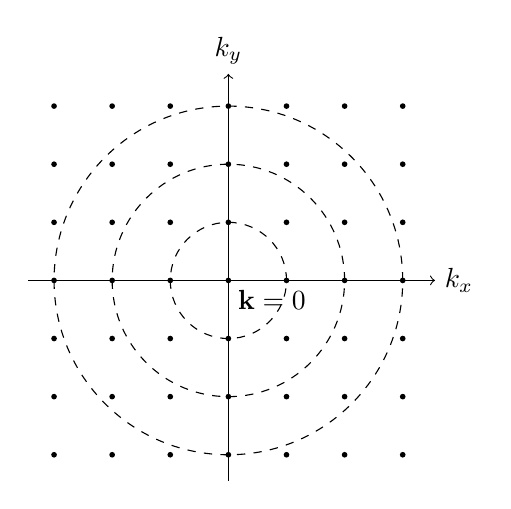
\begin{tikzpicture}[scale=0.82]
\draw[->] (-3.1,0) -- (3.2,0) node[right] {$k_x$};
\draw[->] (0,-3.1) -- (0,3.2) node[above] {$k_y$};
\draw[dashed] (0,0) circle (0.9);
\draw[dashed] (0,0) circle (1.8);
\draw[dashed] (0,0) circle (2.7);
\foreach \x in {-3,-2,-1,0,1,2,3}{
  \foreach \y in {-3,-2,-1,0,1,2,3}{
    \fill (0.9*\x,0.9*\y) circle (1.25pt);
  }
}
\node[below right] at (0,0) {$\mathbf{k}=0$};
\end{tikzpicture}
\caption{有限週期盒中粒子的離散動量態與等能殼層。}
\end{figure}

對於非相對論性粒子，
\begin{equation}
E_{\mathbf{k}}=\frac{\mathbf{k}^2}{2m},
\end{equation}
所以最低能量態是\(\mathbf{k}=0\)。將\(N\)個全同玻色子放入盒中，求其多粒子基態。第一個玻色子進入零動量態。第二個也可以進入同一個態，第三個以及之後的每一個玻色子也都可以。因此，全部\(N\)個玻色子都佔據\(\mathbf{k}=0\)。

這就是玻色子凝聚體：大量全同粒子佔據同一個單粒子態；此處所指的態是最低能量態。零動量波函數在空間中為常數，並遍布整個盒子。它不會將任何一個玻色子局域在特定位置，因此每個玻色子的位置都是不確定的。當佔據數很大時，共同波函數會形成宏觀的場振幅，場的行為也會愈來愈像經典場。

費米子的基態則截然不同。暫且忽略自旋，因此每個動量點代表一個可用態。第一個費米子進入\(\mathbf{k}=0\)，但第二個全同費米子不能再佔據同一態。後續粒子必須佔據能量次低的殼層。在二維示意圖中，離原點最近的非零點陣位置有四個，能量相同；在三維中則有六個。這些態佔滿後，更多粒子就必須進入更外側的殼層。

由於能量正比於動量空間中到原點距離的平方，總能量要最小，就必須在不違反不相容原理的前提下，讓佔據的點盡可能緊密地環繞\(\mathbf{k}=0\)排列。費米子數量很多時，佔據區域近似為球形。其邊界稱為費米面，內部稱為費米海，而整個填滿的區域稱為費米球。有限體積下，可用點構成點陣，因此邊界會略有參差；但對大型系統而言，這項細節可以忽略。

\begin{figure}
\centering
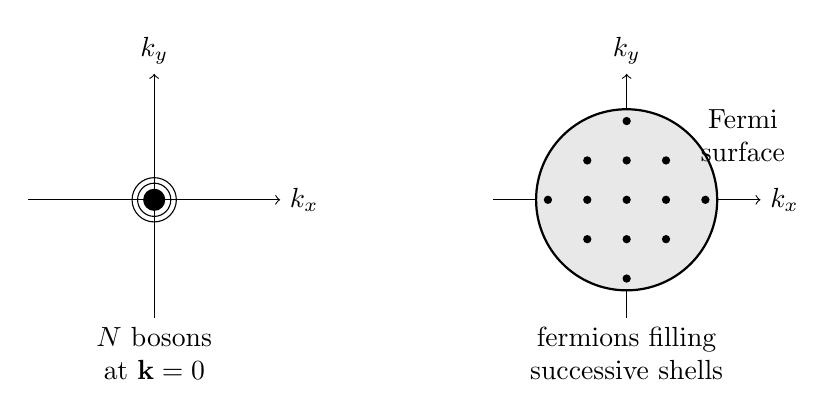
\begin{tikzpicture}[scale=1.0]
\begin{scope}[xshift=-3.0cm]
\draw[->] (-1.6,0) -- (1.6,0) node[right] {$k_x$};
\draw[->] (0,-1.5) -- (0,1.6) node[above] {$k_y$};
\fill (0,0) circle (4pt);
\draw (0,0) circle (6pt);
\draw (0,0) circle (8pt);
\node[align=center] at (0,-1.95) {$N$ bosons\\at $\mathbf{k}=0$};
\end{scope}
\begin{scope}[xshift=3.0cm]
\draw[->] (-1.7,0) -- (1.7,0) node[right] {$k_x$};
\draw[->] (0,-1.5) -- (0,1.6) node[above] {$k_y$};
\fill[gray!18] (0,0) circle (1.15);
\draw[thick] (0,0) circle (1.15);
\fill (0,0) circle (1.5pt);
\fill (0.5,0) circle (1.5pt);
\fill (-0.5,0) circle (1.5pt);
\fill (0,0.5) circle (1.5pt);
\fill (0,-0.5) circle (1.5pt);
\fill (0.5,0.5) circle (1.5pt);
\fill (0.5,-0.5) circle (1.5pt);
\fill (-0.5,0.5) circle (1.5pt);
\fill (-0.5,-0.5) circle (1.5pt);
\fill (1,0) circle (1.5pt);
\fill (-1,0) circle (1.5pt);
\fill (0,1) circle (1.5pt);
\fill (0,-1) circle (1.5pt);
\node[right,align=center] at (0.82,0.82) {Fermi\\surface};
\node[align=center] at (0,-1.95) {fermions filling\\successive shells};
\end{scope}
\end{tikzpicture}
\caption{玻色子凝聚在零動量態；費米子則由內向外填滿動量態，直到費米面。}
\end{figure}

費米子基態的能量遠高於相應的玻色子基態。所有玻色子都能留在零動量態，但大多數費米子不得不佔據非零動量態。加入的費米子愈多，佔據態的最大動量也愈大。此外，高動量處的殼層比原點附近的殼層包含更多點陣位置。因此，大型費米球中有許多粒子具有相當大的動量，處於最低動量態的粒子則只有少數。

這種差異在激發態中也看得出來。對玻色子而言，第一個激發態可由下列方式得到：從凝聚體中取出任意一個玻色子，並將它放入第一個激發單粒子態：
\begin{equation}
(N,0,0,\ldots)\longrightarrow (N-1,1,0,\ldots).
\end{equation}
移動哪一個玻色子都沒有差別，因為粒子彼此全同。較高能量的激發態則有幾種形成方式。依能階間距而定，可以將一個玻色子放入更高能階，或將兩個玻色子放入第一激發能階。激發玻色子系統，就是將粒子從凝聚體提升到較高能量的態。

對費米子而言，不能把任何粒子移至已填滿的費米球內部的其他點，因為那些點都已被佔據。可以從費米海深處取出一個費米子，再將它放到費米面之外，但這需要付出很大的能量。代價最低的激發，是將費米面內側附近的一個費米子移至外側附近的未佔據態。被提升的電子能量只略高於費米面，而留下的空態能量則只略低於費米面。

\begin{figure}
\centering
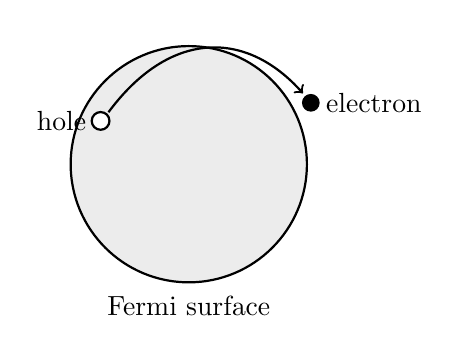
\begin{tikzpicture}[scale=1.0]
\fill[gray!15] (0,0) circle (1.5);
\draw[thick] (0,0) circle (1.5);
\draw[fill=white,thick] (-1.12,0.55) circle (3.2pt);
\fill (1.55,0.78) circle (3.2pt);
\draw[->,thick] (-1.02,0.66) .. controls (-0.25,1.7) and (0.72,1.72) .. (1.45,0.9);
\node[left] at (-1.18,0.55) {hole};
\node[right] at (1.62,0.78) {electron};
\node[below] at (0,-1.55) {Fermi surface};
\end{tikzpicture}
\caption{低能費米子激發會使一個電子躍遷到費米面之外，並留下空穴。}
\end{figure}

\section{空穴與低能激發}

為了具體說明空穴的電荷，設想盒中有正電荷均勻分布於整個體積。在物質中，這些正電荷最終來自原子核中的質子；假設它們均勻分布，則可簡化模型。加入足量電子以中和背景電荷。在基態中，這些電子會填滿費米球。

將一個電子從費米面下方提升到上方，不會改變盒子的總電荷。這會在費米面上方產生一個帶負電的電子，並在下方留下缺少負電荷的空位。因此，可以把缺少的電子視為帶正電的激發，稱為空穴。

\begin{classroomqa}
\lecturetimestamp{01:31:38}
\audiencequestion{費米面下方的空穴具有負能量嗎？}
\lecturerresponse{不會。空穴是相對於多體基態的激發，因此其激發能為正。若能量是以費米面為基準來量度，從費米面下方移除一個已佔據的電子，就需要付出正能量。}
\end{classroomqa}

設移除的電子能量為\(\varepsilon<\varepsilon_F\)，提升後的電子能量為\(\varepsilon'>\varepsilon_F\)。所提供的能量可分解為兩段相對於費米面的正能量差。\footnote{這兩段能量差分別列出；此處呈現的緊湊等式則是代數上等價的重組形式。}
\begin{equation}
\Delta E
=\varepsilon'-\varepsilon
=(\varepsilon'-\varepsilon_F)+(\varepsilon_F-\varepsilon).
\end{equation}
第一項可自然地歸於費米面上方的電子，第二項則歸於下方的空穴：
\begin{equation}
E_{\mathrm{electron}}=\varepsilon'-\varepsilon_F>0,
\qquad
E_{\mathrm{hole}}=\varepsilon_F-\varepsilon>0.
\end{equation}
電子帶負電，空穴帶正電。

費米面上方的電子之後可能落入可用的空穴。電子能量因而降低，釋出的能量必須以輻射帶走。這個過程可以描述為：電子落入較低的未佔據態，並發射一個或多個光子。等價地，也可以說電子與空穴湮滅，轉化為輻射。空穴不是盒中額外的基本組成；它是填滿的多電子態中的缺失。儘管如此，由於它具有能量與電荷，將它視為類粒子激發仍然很有用。

\begin{classroomqa}
\lecturetimestamp{01:36:52}
\audiencequestion{激發電子是否表示在動量空間中將它從一個點陣點移到另一個點陣點？}
\lecturerresponse{這表示將電子從一個能階移至另一個能階。對盒中的自由粒子而言，動量點陣標示了這些能階，但這個概念不依賴動量空間中存在點陣。在原子中，正電荷集中於原子核。電子會填入最低的可用原子能階；光子則能將一個電子提升至激發能階，並在它原先佔據的能階留下空位。這個空位就是原子中的空穴對應物。}
\end{classroomqa}

在盒中，吸收光子同樣會將光子能量轉化為費米面上方的一個電子，以及下方的一個空穴。在原子中，同樣的說法描述了被激發的電子，以及在原先被佔據的較低能階中留下的空位。

\begin{classroomqa}
\lecturetimestamp{01:39:16}
\audiencequestion{費米球中任何位置的電子都能吸收低能光子嗎？}
\lecturerresponse{不能。如果電子位於費米海深處，附近的態都已被佔據，低能光子便無法提供足夠能量，讓它躍遷至費米面上方的未佔據態。只有靠近費米面的電子，才有光子能量範圍內可到達的空態。能量足夠高的光子則能激發深處的電子。}
\end{classroomqa}

因此，低能吸收截面取決於費米海的表面，而非整個體積。費米海深處的電子無法發生小幅躍遷；費米面下方附近的電子則可以躍遷到其上方附近。

\begin{classroomqa}
\lecturetimestamp{01:40:42}
\audiencequestion{沒有入射光子時，有什麼能阻止電子彼此直接作用？}
\lecturerresponse{沒有任何東西。在這個簡單模型中，我們忽略電子--電子的相互作用，因為納入這些作用會使費米海圖像更加複雜。在這個金屬的初步近似模型中，其有效影響被視為足夠微弱，通常可以忽略。}
\end{classroomqa}

\begin{classroomqa}
\lecturetimestamp{01:41:10}
\audiencequestion{如果一個光子的能量足以激發多個電子，會發生什麼事？}
\lecturerresponse{原則上，任何符合守恆定律的過程都可能發生。光子可以產生多組電子--空穴對：激發兩個電子也會留下兩個空穴。這種過程會產生更多激發，通常比起用相同能量更強烈地激發單一電子，發生機率更低。}
\end{classroomqa}

\begin{classroomqa}
\lecturetimestamp{01:42:06}
\audiencequestion{兩個光子單獨都無法造成激發時，能否同時吸收它們？}
\lecturerresponse{可以。吸收具有機率性；即使每個光子單獨的能量都低於所需能量，只要兩者能量總和足以達到某個可用的激發態，雙光子過程就可能發生。如果可用光子的能量不足以達到任何允許的激發態，光大致上就會穿透這個系統。}
\end{classroomqa}

\editorialnote{此處有一段簡短討論，將吸收的輻射與電子的集體運動連結起來，但無法復原其中的實質細節。唯一能確定的是，這種集體響應比單粒子--空穴圖像更複雜。}

\begin{classroomqa}
\lecturetimestamp{01:43:49}
\audiencequestion{所有電子都帶相同的負電，為何電子--電子相互作用仍被稱為微弱？}
\lecturerresponse{電子處於用來補償電荷的正電背景中。這個背景會屏蔽電子的電荷，在此簡化情況下減弱有效相互作用。相互作用並非不存在；若要處理它，就必須考慮介質的屏蔽響應。}
\end{classroomqa}

\begin{classroomqa}
\lecturetimestamp{01:44:41}
\audiencequestion{之後會討論屏蔽效應嗎？}
\lecturerresponse{會。屏蔽效應很重要，但要等到能更完整地處理相互作用系統時再討論。}
\end{classroomqa}

\section{一維費米海與反粒子}

空穴的構想引出反粒子的概念。同樣的邏輯結構可以從物質中的電子，轉用於相對論量子場及其真空。最簡單的版本是在一個空間維度中，考慮無質量費米場\(\psi(x,t)\)。在光速設為一的單位制中，兩種可能的線性色散關係為
\begin{equation}
\omega=k,
\qquad\text{or}\qquad
\omega=-k.
\end{equation}
以下將明確考慮第一個分支。

\editorialnote{結尾的問答交替提出互不相容的粒子認定。能確定的模型，是一個未具體指明種類、位於一個空間維度中的無質量費米玩具場，且只考慮一個傳播方向。}

對於平面波
\begin{equation}
\psi(x,t)=e^{i(kx-\omega t)},
\end{equation}
其導數為
\begin{equation}
\frac{\partial\psi}{\partial t}=-i\omega\psi,
\qquad
\frac{\partial\psi}{\partial x}=ik\psi.
\end{equation}
因此，\(\omega=k\)等價於以下一階場方程：
\begin{equation}
\frac{\partial\psi}{\partial t}
=-\frac{\partial\psi}{\partial x}.
\end{equation}

\begin{figure}
\centering
\includegraphics[width=0.72\textwidth]{lecture_05_figure_05.png}
\caption{一階場方程的推導開端；其平面波解滿足\(\omega=k\)。}
\lectureframe{01:47:22}
\end{figure}

任何形如\(f(x-t)\)的波形都滿足這個方程，並向右傳播。改變符號則得到
\begin{equation}
\frac{\partial\psi}{\partial t}
=+\frac{\partial\psi}{\partial x},
\end{equation}
其波形\(f(x+t)\)向左傳播。每個一階方程只選出一個傳播方向。假設這個場是費米場，並為了進行空穴論證，假設其中的粒子帶有電荷。

分支\(\omega=k\)立即帶來一個困難。波數\(k\)可以為負，因此\(\omega\)也可能為負。由於在這些單位制中，\(\omega\)就是能量，這條直線譜同時包含正能量態與負能量態：
\begin{equation}
E=\omega=k.
\end{equation}

\begin{figure}
\centering
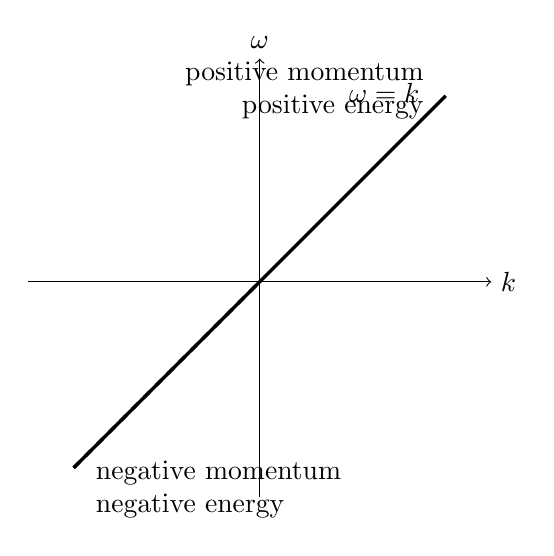
\begin{tikzpicture}[scale=1.05]
\draw[->] (-2.8,0) -- (2.8,0) node[right] {$k$};
\draw[->] (0,-2.6) -- (0,2.7) node[above] {$\omega$};
\draw[very thick] (-2.25,-2.25) -- (2.25,2.25);
\draw[very thick,dashed] (-2.25,-2.25) -- (0,0);
\node[above left] at (2.05,2.05) {$\omega=k$};
\node[below right,align=left] at (-2.1,-2.05) {negative momentum\\negative energy};
\node[above left,align=right] at (2.1,1.85) {positive momentum\\positive energy};
\end{tikzpicture}
\caption{單分支譜\(\omega=k\)；其負能量半支位於\(k<0\)。}
\end{figure}

在這種理論中，通常所說的空真空不可能是基態。正能量費米子可以輻射光子並躍遷到較低能態。沒有任何機制會使它在零能量處停下來：它可以繼續進入負能量態，發射更多輻射，能量也就不斷降低。費米子失去的能量會出現在輻射場中。因此，能量下方無界的譜無法提供穩定的普通真空。

費米子的排他性提供了另一種出發點。將所有負能量單粒子態一路填入費米子，直到零能量為止。這些態都已被佔據，因此沒有其他費米子能再躍遷進去。既然無法再加入負能量費米子，而加入正能量費米子又會提高能量，完全填滿的負能量海便可作為多體基態，並稱為真空。

\begin{figure}
\centering
\resizebox{\linewidth}{!}{%
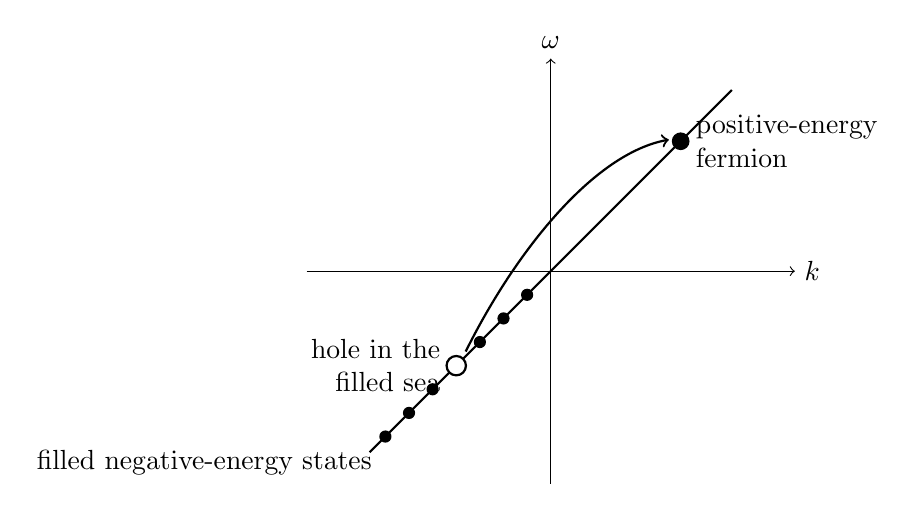
\begin{tikzpicture}[scale=1.0]
\draw[->] (-3.1,0) -- (3.1,0) node[right] {$k$};
\draw[->] (0,-2.7) -- (0,2.7) node[above] {$\omega$};
\draw[thick] (-2.3,-2.3) -- (2.3,2.3);
\foreach \p in {-2.1,-1.8,-1.5,-1.2,-0.9,-0.6,-0.3}{
  \fill (\p,\p) circle (2.2pt);
}
\draw[fill=white,thick] (-1.2,-1.2) circle (3.5pt);
\fill (1.65,1.65) circle (3.2pt);
\draw[->,thick] (-1.08,-1.02) .. controls (-0.45,0.25) and (0.55,1.5) .. (1.5,1.67);
\node[left,align=right] at (-1.28,-1.2) {hole in the\\filled sea};
\node[right,align=left] at (1.72,1.65) {positive-energy\\fermion};
\node[below left] at (-2.15,-2.15) {filled negative-energy states};
\end{tikzpicture}%
}
\caption{填滿負能量海的狀態，以及將一個費米子提升至正能量態所形成的激發。}
\end{figure}

最簡單的激發，是從負能量海中移除一個費米子，並將它放入正能量態。被提升的費米子是普通的正能量粒子。海中留下的空位則是另一種激發，也就是空穴。如果被移除的費米子帶負電，空穴便帶正電。

在這個單分支例子中，空穴也具有正動量。假設缺失的費米子原本佔據動量為\(k_-<0\)的態，移除它會使總動量改變
\begin{equation}
p_{\mathrm{hole}}=-k_->0.
\end{equation}
這代表負動量的缺額。因此，這個激發由一個正能量、帶負電的費米子，以及一個正能量、帶正電的空穴組成。兩者都帶有正動量，而且在\(\omega=k\)分支上都向右傳播。

在完整的電子理論中，帶正電的空穴就是正電子。狄拉克最初曾考慮將空穴認定為質子。這種構造要求粒子與其反粒子具有相同質量。空穴是一種不同的粒子，其質量與電子相同，電荷則與電子相反。這就是負能量譜所引出的基本粒子--反粒子詮釋。

同樣的解決方式無法用於玻色子。玻色子態可以容納任意多個粒子，因此無法只填入一個粒子就封住負能量態，阻止其他粒子進入。還是可以不斷加入更多玻色子，使能量一次又一次降低：
\begin{equation}
\begin{aligned}
\text{fermionic mode: }&n=0\ \text{or}\ 1,\\
\text{bosonic mode: }&n=0,1,2,\ldots .
\end{aligned}
\end{equation}
這個假設的玻色子系統仍然沒有基態。在這個基本構造中，填滿負能量海之所以穩定，正是依賴費米子的排他性。

這個一維方程只是狄拉克方程的玩具版本。它描述的場沒有質量，以光速運動，且只沿一個方向傳播。更完整的狄拉克方程必須涵蓋此處缺少的運動方向，以及相對論性粒子結構的其他部分。這個更完整的方程，以及玻色子場中反粒子的處理方式，都留待後續討論。
